% Appendix Template

\chapter{Results of experiment 2.4} % Main appendix title

\label{Appendix2-4} % Change X to a consecutive letter; for referencing this appendix elsewhere, use \ref{AppendixX}

\begin{figure}[th]
\centering
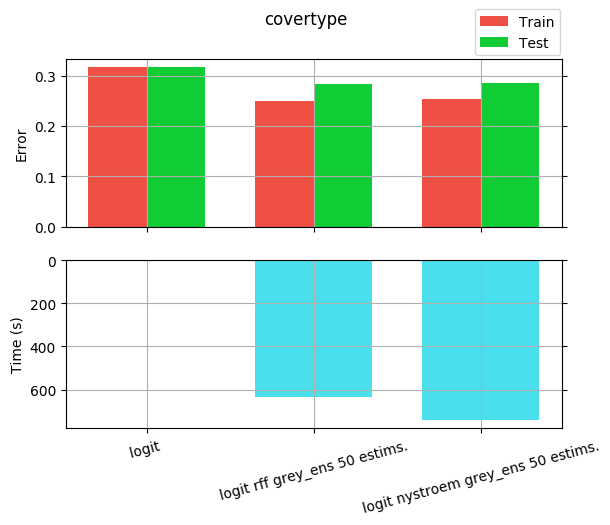
\includegraphics[scale=\imgscale]{Figures/2_4/covertype}
\decoRule
\caption[2.4 covertype]{Logistic Regression with Grey Ensemble model}
\label{fig:2_4_covertype}
\end{figure}

\begin{figure}[th]
\centering
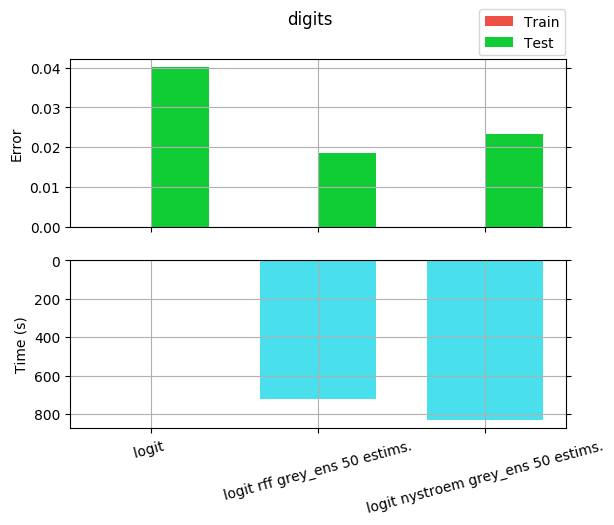
\includegraphics[scale=\imgscale]{Figures/2_4/digits}
\decoRule
\caption[2.4 digits]{Logistic Regression with Grey Ensemble model}
\label{fig:2_4_digits}
\end{figure}

\begin{figure}[th]
\centering
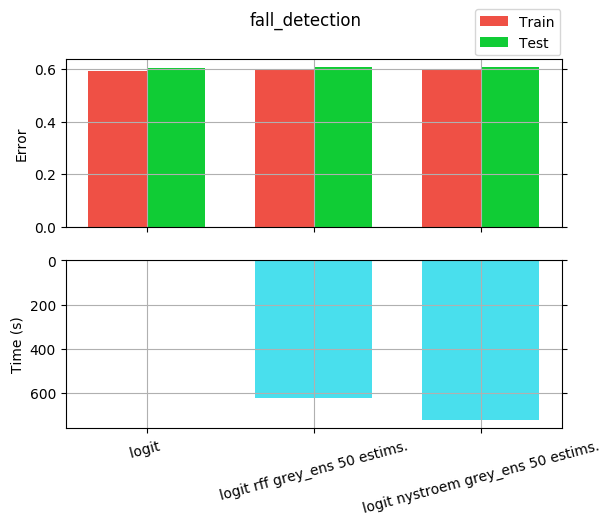
\includegraphics[scale=\imgscale]{Figures/2_4/fall_detection}
\decoRule
\caption[2.4 fall\tu detection]{Logistic Regression with Grey Ensemble model}
\label{fig:2_4_fall_detection}
\end{figure}

\begin{figure}[th]
\centering
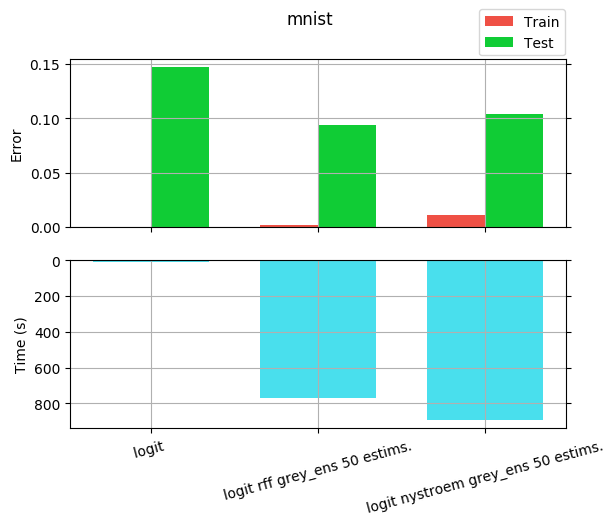
\includegraphics[scale=\imgscale]{Figures/2_4/mnist}
\decoRule
\caption[2.4 mnist]{Logistic Regression with Grey Ensemble model}
\label{fig:2_4_mnist}
\end{figure}

\begin{figure}[th]
\centering
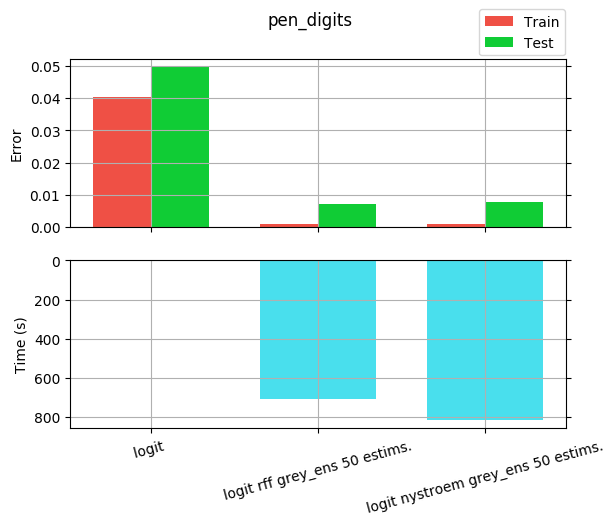
\includegraphics[scale=\imgscale]{Figures/2_4/pen_digits}
\decoRule
\caption[2.4 pen\tu digits]{Logistic Regression with Grey Ensemble model}
\label{fig:2_4_pen_digits}
\end{figure}

\begin{figure}[th]
\centering
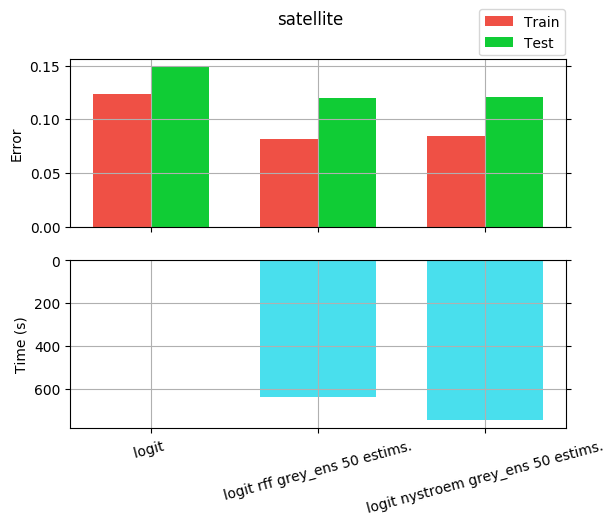
\includegraphics[scale=\imgscale]{Figures/2_4/satellite}
\decoRule
\caption[2.4 satellite]{Logistic Regression with Grey Ensemble model}
\label{fig:2_4_satellite}
\end{figure}

\begin{figure}[th]
\centering
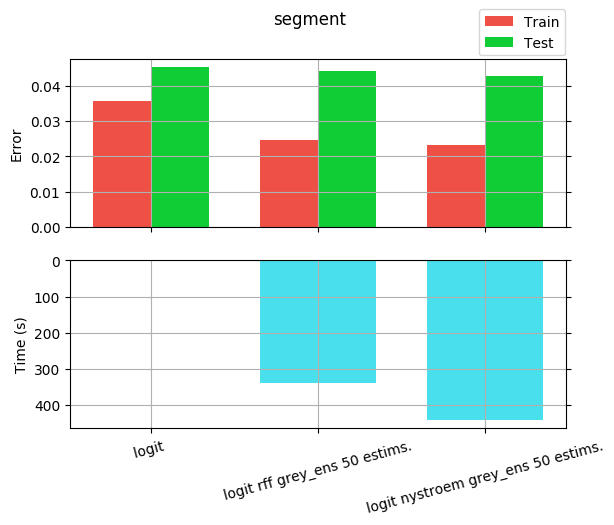
\includegraphics[scale=\imgscale]{Figures/2_4/segment}
\decoRule
\caption[2.4 segment]{Logistic Regression with Grey Ensemble model}
\label{fig:2_4_segment}
\end{figure}

\begin{figure}[th]
\centering
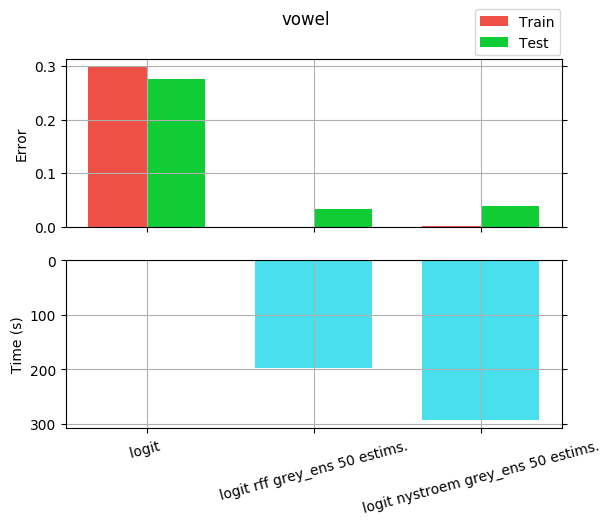
\includegraphics[scale=\imgscale]{Figures/2_4/vowel}
\decoRule
\caption[2.4 vowel]{Logistic Regression with Grey Ensemble model}
\label{fig:vowel}
\end{figure}
